\chapter{Evaluation des besten Lösungsansatzes}
\label{ch:evaluation-loesungsansatz}

Aufbauend auf den beiden vorangegangenen Kapiteln, in denen Lösungsansätze entworfen und die Implementierung
beschrieben wurde, konnte ein Vorgehen zur Auswahl der besten \ac{KI}-Strategie entwickelt werden, auf die in diesem
Kapitel eingegangen wird.

\section{Vorgehen zur Auswahl der besten Strategie}
\label{sec:auswahl-strategie}

Die Überlegung hierbei war es, basierend auf der in \Kapitel{sec:offline-implementierung} beschriebenen
Möglichkeit, Spiele auch ohne Zugriff auf den spe\_ed-Server mit mehreren unserer \ac{KI}s ausführen zu können,
eine automatisierte Simulation möglichst vieler Spiele durchführen zu können.
Die daraus resultierenden Ergebnisse sollten in einer Form gespeichert werden, die es im Anschluss ermöglicht, daraus
Informationen über die Stärke einer bestimmten \ac{KI} mit ihren unterschiedlichen Konfigurations-Möglichkeiten gewinnen
zu können. \\

Zu diesem Zweck wurde die Klasse \Code{AIEvaluationController} erstellt, der vom bereits erläuterten
\Code{OfflineController} erbt.
Dieser ruft bei der Ausführung in einer Schleife die \Code{play}-Methode des \Code{OfflineController} auf, wobei bei
jedem Aufruf ein neues Spiel generiert wird.
Hierbei mussten allerdings einige Annahmen getroffen werden, die potenziell einen Einfluss auf das Ergebnis haben
könnten:

\begin{itemize}
    \item Ein Spielfeld besitzt bei der Simulation eine zufällige Höhe und Breite zwischen 30 und 70 Feldern.
    \item Den \ac{KI}s wird für die Auswahl in einer Runde eine zufällige Zeit zwischen 3 und 15 Sekunden eingeräumt.
    \item Es nehmen an einem Spiel immer eine zufällige Anzahl an Spielern teil, die zwischen 3 und 6 liegen kann.
\end{itemize}

Nach jeder Berechnung einer \ac{KI} wird die Berechnungsdauer abgespeichert.
Gleiches wird nach dem Ende eines jeden Spiels für das Spiel selber und die teilnehmenden Spieler durchgeführt, wobei
auch die Information über den Sieger eines Spiels erhalten bleibt.

\section{Entwurf einer \acL{DB} zum Speichern der Simulationen}
\label{sec:entwurf-datenbank}

Um die beschriebenen Daten leicht abfragen zu können, fiel die Entscheidung auf die Nutzung einer relationalen
\ac{DB}.
In diesem Fall wurde dafür SQLite3 ausgewählt, da die gesamte \ac{DB} in einer Datei gespeichert wird und somit das
Aufsetzen eines \acl{DB}-Managements-Systems entfällt. \Vgl{sqlite3}
Die Verbindung konnte dann mit der Python-Bibliothek \Code{sqlite3} \Vgl{python-sqlite3} hergestellt werden.
Zuerst aber war es notwendig, die \ac{DB}-Struktur zu entwerfen, um anschließend entsprechende SQL-Statements im Code
auf die \ac{DB} anwenden zu können.

\subsection{Erstellen des \acl{ER}-Modells}
\label{subsec:er-modell}

Im ersten Schritt wurde dazu ein \ac{ER}-Modell basierend auf den zugrunde liegenden Anforderung entworfen.
Wie bereits beschrieben, wollen wir primär Informationen erhalten, wie oft eine
bestimmte \ac{KI} mit welchen Parametern in den simulierten Spielen gewonnen hat.
Ziel dieser Evaluation war es nicht, das Verhalten der \ac{KI} in bestimmten Spielsituationen zu beurteilen,
sondern die Qualität der Folge aller Entscheidungen einer \ac{KI} in einem Spiel zu beurteilen.
Die \ac{KI}, die die beste Folge von Entscheidungen getroffen hat sollte gewonnen haben, sodass wir die Anzahl
gewonnener Spiele als Maßzahl für die Stärke der \ac{KI} gewählt haben.
Ein weiterer wichtiger Wert stellt die durchschnittliche Ausführungsdauer einer \ac{KI} dar und diesen \ua
mit der Spielfeldgröße und der Anzahl der am Spiel teilnehmenden Gegnern in Korrelation bringen zu können.
Das daraus resultierende \ac{ER}-Modell ist in \Abbildung{fig:er-schema} dargestellt.

\begin{figure}[htb]
	\centering
	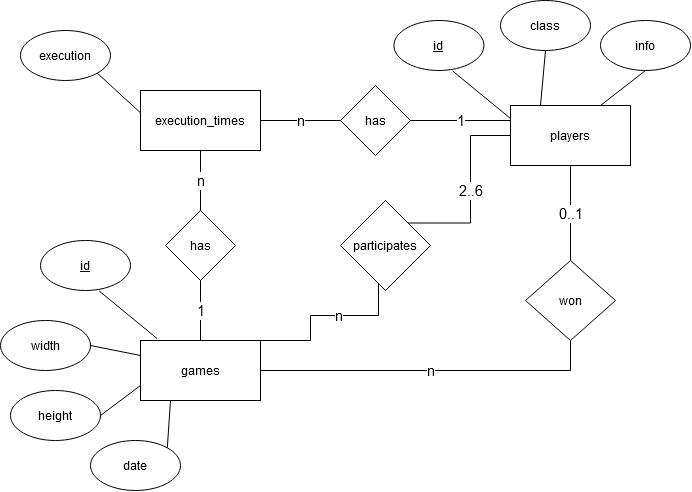
\includegraphics[width=0.9\textwidth]{Bilder/er-diagram.png}
	\caption{\ac{ER}-Modell der Evaluations-\ac{DB}}
	\label{fig:er-schema}
\end{figure}

\subsection{Überführen des \ac{ER}-Modells in ein relationales \acl{DB}-Modell}
\label{subsec:db-schema}

Das \ac{ER}-Modell wurde anschließend in ein relationales Modell überführt, welches die tatsächlichen Relationen in der
Datenbank darstellt.
Dazu wurden Primärschlüssel festgelegt und über Fremdschlüssel Verknüpfungen zwischen den Relationen hergestellt.
Bei der Modellierung wurde darauf geachtet, die dritte Normalform der \ac{DB}-Normalisierung einzuhalten,
um Anomalien und Redundanzen zu verhindern.
\Vgl{db-normalisierung}
In \Abbildung{fig:relationales-db-schema} ist das entworfene relationale Modell zu sehen.

\begin{figure}[htb]
	\centering
	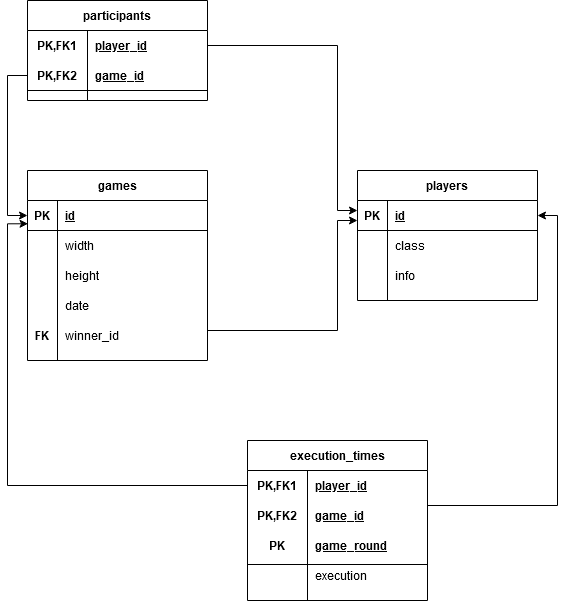
\includegraphics[width=0.7\textwidth]{Bilder/relationales_db_schema.png}
	\caption{Relationales Datenbankschema der Evaluations-Datenbank}
	\label{fig:relationales-db-schema}
\end{figure}

\section{Ergebnis der Evaluation}
\label{sec:ergebnis-evaluation}

Die Evaluation wurde in zwei Etappen durchgeführt.
Für den ersten Teil der Evaluation wurden alle implementierten \ac{KI}s in verschiedenen Konfigurationen für die Simulation betrachtet.
Aufbauend auf diesen Ergebnissen wurde eine zweite Simulation gestartet, in der nur die besten \ac{KI}s berücksichtigt
wurden.

\subsection{Ergebnisse der ersten Evaluation}
\label{subsec:erste-evaluation}

Mit dem oben beschriebenen \Code{AIEvaluationController} wurden in einem Zeitraum von 16 Tagen insgesamt 1000 Spiele
mit zufälligen \ac{KI}-Konstellationen simuliert und dabei insgesamt 638685 Spielzüge berechnet.
Um aus den gespeicherten Daten der \ac{DB} die besten \ac{KI}s herauszufiltern, wurde insbesondere jeweils die
Siegquote in den Spielen betrachtet, an denen sie teilgenommen haben.
Mit dem in \Anhang{lst:eval-sql-1} abgebildetem SQL-Statement wird eine solche Quote gruppiert nach der \ac{KI}-Klasse
berechnet.
Das Ergebnis kann der \Tabelle{tab:evaluation-ki-klasse} entnommen werden.

\begin{table}[htb]
    \centering
    \begin{tabularx}{\textwidth}{|X|c|c|c|c|c|c|c|}
        \hline
		\textbf{Klasse} & \textbf{Wins} & \textbf{Plays} & \textbf{Gewinn-}   & \textbf{Max}   & \textbf{Avg}   & \textbf{Avg}     & \textbf{Deadline} \\
                        &               &                & \textbf{rate (\%)} & \textbf{Zeit}  & \textbf{Zeit}  & \textbf{Zeit oD} & \textbf{eingehal-} \\
                        &               &                &                    & \textbf{(Sek)} & \textbf{(Sek)} & \textbf{(Sek)}   & \textbf{ten (\%)} \\ \hline
        Not\-Killing\-Itself\-AI & 149 & 491 & 30.35 & 1.5989 & 0.3621 & 0.3568 & 100 \\ \hline
        Path\-finding\-AI & 303 & 1000 & 30.3 & 60.001 & 4.3782 & 2.1739 & 96.19 \\ \hline
		Path\-finding\-Search\-Tree\-AI & 297 & 1000 & 29.7 & 60.002 & 9.3117 & 2.6884 & 88.44 \\ \hline
		Search\-Tree\-Path\-finding\-AI & 238 & 1000 & 23.8 & 60.002 & 6.6962 & 2.24 & 92.28 \\ \hline
		Search\-Tree\-AI & 6 & 733 & 0.82 & 60.002 & 4.2471 & 0.3472 & 93.46 \\ \hline
		Random\-AI & 0 & 257 & 0 & 0.0251 & 0.0078 & 0.0078 & 100 \\ \hline
    \end{tabularx}
    \caption{Auswertung der besten \ac{KI}-Klasse}
    \label{tab:evaluation-ki-klasse}
\end{table}

Etwas überraschend hat die \Code{NotKillingItselfAI} demnach am besten abgeschnitten, obwohl andere Taktiken wie bereits
erläutert teilweise hierauf aufbauen und die Ermittlung der besten Aktion um zusätzliche Berechnungen erweitern.
Um ein differenzierteres Ergebnis zu erhalten, wurde die Abfrage aus \Anhang{lst:eval-sql-2} ausgeführt, welche
nicht nur die Art der \ac{KI}, sondern zusätzlich auch ihre jeweiligen Konfigurationsparameter betrachtet.
In \Tabelle{tab:evaluation-ki-konfiguration} werden die ersten Einträge reduziert auf die relevantesten Spalten
abgebildet.

\begin{table}[htb]
    \centering
    \begin{tabularx}{\textwidth}{|X|X|c|c|c|}
        \hline
		\textbf{Klasse} & \textbf{Info} & \textbf{Wins} & \textbf{Plays} & \textbf{Gewinn-} \\
                        &               &               &                & \textbf{rate (\%)} \\ \hline
        Path\-finding\-Search\-Tree\-AI & max\_""speed""=""1, paths\_""tolerance""=""0.75, count\_""paths\_""to\_""check""=""50, depth""=""2, distance\_""to\_""check""=""30 & 12 & 18 & 66.67 \\ \hline
        Search\-Tree\-Path\-finding\-AI & max\_""speed""=""1, count\_""paths\_""to\_""check""=""25, depth""=""2, distance\_""to\_""check""=""20 & 17 & 26 & 65.38 \\ \hline
        Path\-finding\-Search\-Tree\-AI & max\_""speed""=""1, paths\_""tolerance""=""0.75, count\_""paths\_""to\_""check""=""25, depth""=""2, distance\_""to\_""check""=""10 & 10 & 16 & 62.50 \\ \hline
        Path\-finding\-Search\-Tree\-AI & max\_""speed""=""1, paths\_""tolerance""=""0.75, count\_""paths\_""to\_""check""=""75, depth""=""3, distance\_""to\_""check""=""10 & 7 & 12 & 58.33 \\ \hline
        Path\-finding\-Search\-Tree\-AI & max\_""speed""=""2, paths\_""tolerance""=""0.75, count\_""paths\_""to\_""check""=""75, depth""=""3, distance\_""to\_""check""=""20 & 8 & 15 & 53.33 \\ \hline
        Path\-finding\-Search\-Tree\-AI & max\_""speed""=""1, paths\_""tolerance""=""0.75, count\_""paths\_""to\_""check""=""75, depth""=""2, distance\_""to\_""check""=""10 & 9 & 17 & 52.94 \\ \hline
        Path\-finding\-AI & max\_""speed""=""1, count\_""paths\_""to\_""check""=""50 & 63 & 120 & 52.50 \\ \hline
        \ldots & \ldots & \ldots & \ldots & \ldots \\ \hline
    \end{tabularx}
    \caption{Auswertung der besten \ac{KI}-Konfiguration}
    \label{tab:evaluation-ki-konfiguration}
\end{table}

Hierbei wird deutlich, dass die \Code{NotKillingItselfAI} schlechter abschneidet als es das erste SQL-Statement vermuten ließ.
Das liegt daran, dass die anderen Implementierungen abhängig von der Konfiguration deutlich besser, aber eben auch
deutlich schlechter abschneiden können.
Dies kann an den komplexeren Berechnungen liegen, die je nach Zustand des Spiels nicht innerhalb der Deadline
abgeschlossen werden können und dann eine schlechte Bewegung durch eine fehlende Rückmeldung an den Server zur Folge
haben. \\

Weitere Erkenntnisse, die aus dem Ergebnis gezogen werden konnten, waren \ua, dass die Anzahl der Felder, die von der
\Code{PathfindingAI} geprüft werden, sehr deutlich unter der Anzahl aller Felder liegen kann.
Die beste Konfiguration prüft nur zu 50 Feldern die Pfade, während ein Spielfeld aus mindestens $30 * 30 = 900$ Feldern
besteht.
Außerdem ist zu sehen, dass besonders \ac{KI}s mit einer niedrigen Maximal-Geschwindigkeit von 1 oder 2 gute Ergebnisse
erzielen.

\subsection{Ergebnisse der zweite Evaluation}
\label{subsec:zweite-evaluation}

Anschließend wurden die besten 25 Konfigurationen, die wir als Ergebnis in der \Tabelle{tab:evaluation-ki-konfiguration}
erhalten haben, hart in einem Array codiert.
Die Spielerstellung wurde zur ersten Evaluation dahingehend angepasst, dass nicht mehr zufällige \ac{KI}s für die
Spieler gewählt wurden, sondern die zufällige Auswahl auf die Einträge dieses Arrays beschränkt wurde.

\todo{Kapitel ausformulieren}
